\section{OOD}
\subsection{Ziel des Entwurfs}
  \begin{itemize}[leftmargin=0.5cm]
    \item Spezifizierte Anwendung auf einer Plattform unter den gefordeten technischen
      Randbedinungen zu ralisieren
    \item Entwurf liegt noch in einem höheren Abstaktionsniveau als in der Implementierung
    \item In der Entwurfsphase wird das OOD-Modell unter den Gesichtspunkten
      der Effizienz und Standartisierung konzipiert.
    \item Jede entworfene Klasse kann direkt implementiert werden
    \item Das OOD-Modell baut auf dem OOA-Modell auf
    \item Die Namen in dem OOD-Modell sollten der Syntax der jeweiligen Progarmmiersprache
      entsprechen.
  \end{itemize}

  \parbox{9cm}{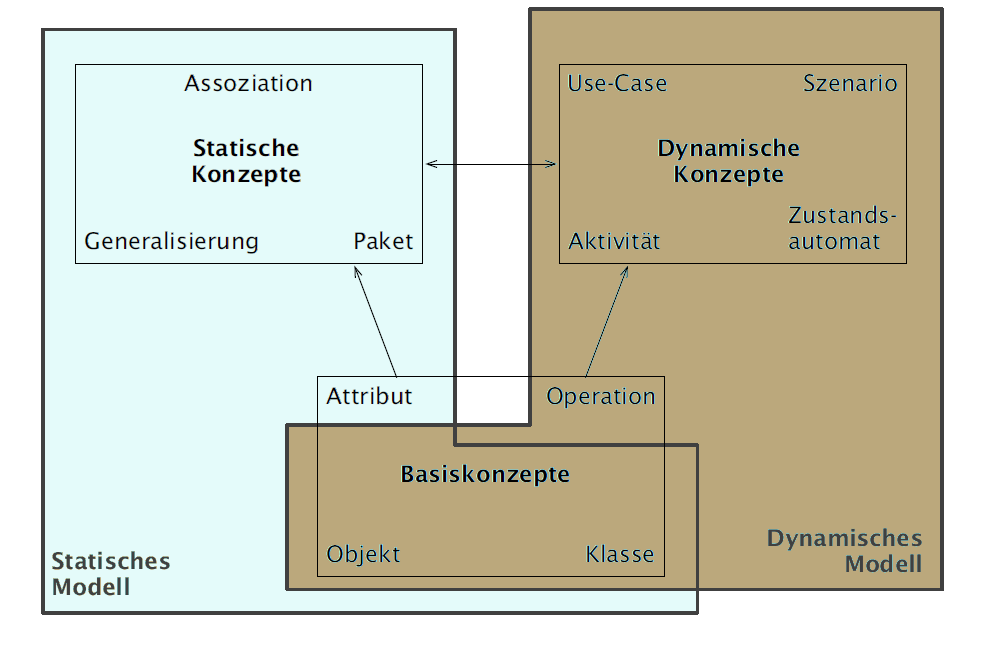
\includegraphics[width=9cm]{./bilder/Konzepte.png}}
  
\subsection{Klassen \balzert{252}}
  \begin{description}
    \item[parametrisierte Klasse]
      Template
    \item[Container Klasse]
      dient zur Verwaltung von einer Menge von Objekten einer anderen Klasse
      (typischerweise als Array implementiert)
    \item[Schnittstelle]
      \parbox{5cm}{ähnlich wie abstrakte Klasse, aber \textbf{keine Operation} ist implementiert}
      \hspace{0.5cm}
      \parbox{3.5cm}{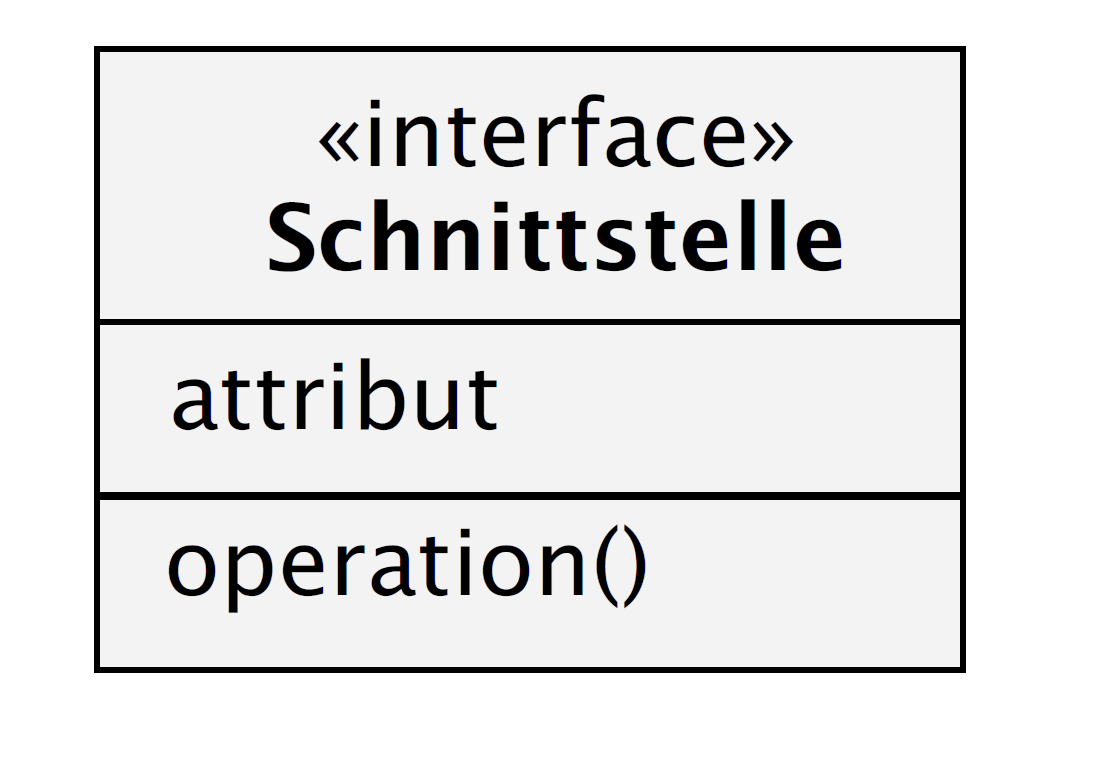
\includegraphics[width=3.5cm]{./bilder/Schnittstelle.png}}
    \item[Implementierung]
      siehe \Balzert{258, 259}
  \end{description}
  

\subsection{Attribut \balzert{261}}
  \begin{description}
    \item[Sichtbarkeit]
      \begin{itemize}[leftmargin=0.5cm]
        \item[$+$] public
        \item[$\#$] protected
        \item[$-$] privat
        \item[$\sim$] package
      \end{itemize}
    \item[Klassenattribute]
      werden durch \underline{Unterstrichen} gekennzeichnet und mit \textbf{static} implementiert
    \item[Notation]
      Sichtbarkeit / \textbf{name} : Typ [Multiplizität] = Anfangswert {Eigenschaftswert} \\
    \parbox{6cm}{
      \item[Eigenschaftswerte]
        siehe \Balzert{263}
      \item[Implementation]
        siehe \Balzert{264} }
    \parbox{6cm}{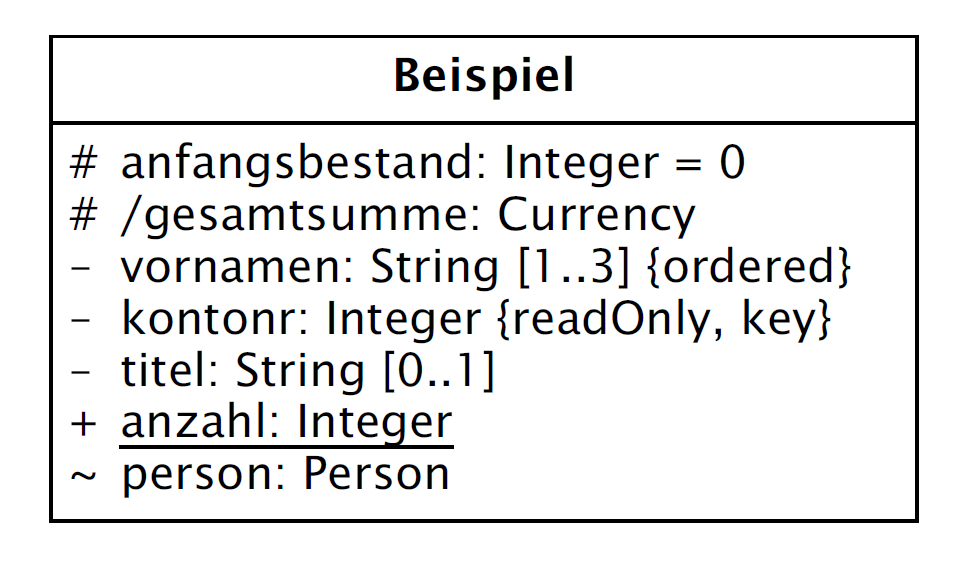
\includegraphics[width=5cm]{./bilder/Notation_Attribute.png}}
  \end{description}
  
  